%
%
%%Text ist für mich noch nicht zufriedenstellend
%In diesem Kapitel geht es um die \emph{Richtcharakteristik von kreisf\"ormigen Antennen}.
%Vorweg genommen bekommt man die \emph{Besselfunktion} als L\"osung.
%Die Herleitung ist aber allgemein f\"ur aller zylindrische K\"orper anwendbar.
%F\"ur das bessere Verst\"andnis wird zuerst der Weg von einer rechteckigen Pauke zu einer kreisf\"ormigen Pauke gemacht und erst danach kommen wir zum Thema \emph{Richtcharakteristik von kreisf\"ormigen Antennen}.
%
%
%
%Potenzreihenherleitung
\section[Potenzreihenherleitung der Besselfunktion]{Potenzreihenherleitung der Besselfunktion 1. Art}
	Das Ziel dieses Abschnittes ist, die Besselfunktion mit der Potenzreihen-Methode die in Kapitel \ref{section:potenzreihen:verallgemeinert} erl\"autert wurde,
	herzuleiten.
\dots \\
%Dieser Abschnitt befasst sich mit der Potenzherleitung der Besselfunktion. 
%Bei der Herleitung werden Methoden, die in den vorherigen Kapitel  erl\"autert wurden, 
%verwendet. Zuerst m\"uss eine Differentialgleichung aufgestellt werden.
%Die Besselfunktion kommt aus der Wellengleichung.
%
	\dots So kommt man auf die Gleichung \refeq{eq:bessel:dgl},
	welche grosse \"Ahnlichkeit mit der Gleichung \refeq{potenzreihen:verallgemeinert-bessel} aufweisst.
%Die Differentialgleichung f\"ur die Besselfunktion lautet wiefolgt:
\begin{align}
	r^2 \, R'' \left( r \right)
	+
	r \, R' \left( r \right)
	+
	\left( r^2 - n^2 \right) \, R \left( r \right)
	=
	0
	\label{eq:bessel:dgl}
\end{align}
	Im Folgenden wird nun die Gleichung \refeq{eq:bessel:dgl},
	mithilfe der Potenzreihen-Methode aus dem Kapitel \ref{section:potenzreihen:verallgemeinert},
	gel\"ost und der L\"osungsweg aufgezeigt.
\subsection[Vorgehensweise]{Vorgehensweise f\"ur die Herleitung der Besselfunktion}
\begin{compactenum}
	\item Die Potenzreihe und deren Ableitungen berechnen.
	\item Die Potenzreihen in die Differentialgleichung \refeq{eq:bessel:dgl} eingesetzen, um
	\item die Indexgleichung f\"ur $\varrho$ zu l\"osen, welche
	\item eine Rekursion der Koeffizienten erm\"oglicht.
	\item Bestimmen der Koeffizienten f\"ur
	\item die Besselfunktion mit ganzzahlige Parametern \refeq{eq:bessel_summenformel}.
%	\item Allgemeine Besselfunktion \refeq{eq:bessel_summenformel:allgemein}
\end{compactenum}


%Um die Differentialgleichung zu l\"osen, w\"ahlen wir den Potenzreihenansatz mit der folgenden Potenzreihe und deren Ableitungen:
\subsection[Potenzreihe und deren Ableitungen]{Potenzreihe und deren Ableitungen berechnen}

\begin{normalsize}
	Wie schon erw\"ahnt,
	kann mit Hilfe der Potenzreihen-Methode die Differentialgleichung \refeq{eq:bessel:dgl} gel\"ost werden.
	F\"ur den Ansatz ben\"otigen wir zuerst eine verallgemeinerte Potenzreihe wie \refeq{eq:bessel:potenzreihe:verallgemeinert}.
	Da in der Differentialgleichung die erste und zweite Ableitung vorkommt,
	muss die Potenzreihe abgeleitet werden,
	was wiederum eine Potenzreihe ergibt,
	wie \refeq{eq:bessel:potenzreihe:ersteableitung} und \refeq{eq:bessel:potenzreihe:zweiteableitung} zeigen.
\end{normalsize}
\\
\begin{align}
	R \left( r \right)
	&=
	r^{\varrho}
	\sum_{k=0}^{\infty} a_k \, r^k
	\label{eq:bessel:potenzreihe:verallgemeinert}
\\
	R'\left( r \right)
	&=
	\varrho \, r^{\varrho - 1}
	\sum_{k=0}^{\infty} a_k \, r^k
	+
	r^{\varrho}
	\sum_{k=0}^{\infty} a_k \, k \, r^{k - 1}
	\label{eq:bessel:potenzreihe:ersteableitung}
\\
	R'' \left( r \right)
	&=
	\varrho \, \left( \varrho - 1 \right) \, r^{\varrho - 2}
	\sum_{k=0}^{\infty} a_k \, r^k
	+
	2 \, \varrho \, r^{\varrho - 1}
	\sum_{k=0}^{\infty} a_k \, k \, r^{k - 1}
	+
	r^{\varrho}
	\sum_{k=0}^{\infty} a_k \, k \, \left( k - 1 \right) \, r^{k - 2}	
	\label{eq:bessel:potenzreihe:zweiteableitung}
\end{align}
%\\
%\begin{normalsize}
%	Wie man sieht,
%	wird die Potenzreihe mit zunehmender Ableitung immer gr\"osser und un\"ubersichtlicher.
%	Zudem verringert sich bei jeder Ableitung der Grad der Potenz um 1.
%	Wenn man die Potenz als Stelle nimmt,
%	dann kann man auch sagen,
%	dass sich pro Ableitung,
%	alle Koeffizienten um eine Stelle nach links verschieben.
%	Dank dieser Verschiebung ist es m\"oglich,
%	eine Abh\"anigkeit bzw. eine Rekursion der Koeffizienten zu erreichen.
%	Mit der Rekursion ist es wiederum m\"oglich,
%	nur wenige der Koeffizienten selber zu definieren m\"ussen,
%	was den Freiheitsgrad reduziert und somit die Berechnung vereinfacht.
%	
%%	\begin{description}[style = nextline, leftmargin = \parindent, labelindent = \parindent]
%%	%[style = multiline, labelwidth = 3.5cm, leftmargin = 3.5cm, itemsep = 1cm]
%%		\item[Wieso ist es ein Vorteil, den Freiheitsgrad zu reduzieren?]
%%		\dots Parameter reduzieren \dots Anzahl M\"oglichkeiten reduzieren \dots \\
%%	\end{description}
%		
%\end{normalsize}

\subsection[Potenzreihen in Differentialgleichung \refeq{eq:bessel:dgl} einsetzen]{Potenzreihen in Differentialgleichung \refeq{eq:bessel:dgl} einsetzen \dots}
%Nun kann man die Potenzreihen in die Differentialgleichung \refeq{eq:bessel:dgl} einsetzen und bekommt dann:
%
%\begin{normalsize}
%	Der n\"achste Schritt ist,
%	die erhaltenen Potenzreihen in die Differentialgleichung \refeq{eq:bessel:dgl} einzusetzen \dots
%\end{normalsize}

\begin{align*}
	\textcolor{mygreen}{r^2 \, R'' \left( r \right)}
	+
	\textcolor{teal}{r \, R' \left( r \right)}
	+
	\textcolor{blue}{\left( r^2 - n^2 \right) \, R \left( r \right)}
	=
	0
	\tag{\ref{eq:bessel:dgl}}
\end{align*}
%
\begin{align*}	
	\textcolor{mygreen}{
		\varrho \, \left( \varrho - 1 \right) \, r^{\varrho}
		\sum_{k=0}^{\infty} a_k \, r^k
		+
		2 \, \varrho \, r^{\varrho}
		\sum_{k=0}^{\infty} a_k \, k \, r^k
		+
		r^{\varrho}
		\sum_{k=0}^{\infty} a_k \, k \, \left( k - 1 \right) \, r^k
	}
	+ \\
	\textcolor{teal}{
		\varrho \, r^{\varrho}
		\sum_{k=0}^{\infty} a_k \, r^k
		+
		r^{\varrho}
		\sum_{k=0}^{\infty} a_k \, k \, r^k
	}
	+ 
	\textcolor{blue}{
		\biggl(
		r^2 - n^2
		\biggr) \,
		r^{\varrho}
		\sum_{k=0}^{\infty} a_k \, r^k
	}
	= & \, 0
\end{align*}
\begin{normalsize}
	\dots , ausmultiplizieren \dots
\end{normalsize}
\begin{align*}
	\textcolor{mygreen}{	\varrho \, \left( \varrho - 1 \right)} 
	\, r^{\varrho}
	\sum_{k=0}^{\infty} a_k \, r^k
	+
	\textcolor{mygreen}{2 \, \varrho}
	\, r^{\varrho}
	\sum_{k=0}^{\infty} a_k \, k \, r^k
	+
	\textcolor{mygreen}{1}
	\, r^{\varrho}
	\sum_{k=0}^{\infty} a_k \, k \, \left( k - 1 \right) \, r^k
	+ \\
	\textcolor{teal}{\varrho}
	\, r^{\varrho}
	\sum_{k=0}^{\infty} a_k \, r^k
	+
	\textcolor{teal}{1}
	\, r^{\varrho}
	\sum_{k=0}^{\infty} a_k \, k \, r^k
	+ 
	r^{\varrho}
		\sum_{k=0}^{\infty} a_k \, r^{k \textcolor{blue}{+ 2}}
	-
	\textcolor{blue}{n^2}
	\, r^{\varrho}
	\sum_{k=0}^{\infty} a_k \, r^k
	= & \, 0
\end{align*}
\\
%Gleiche Summenzeichen zusammenfassen:
\begin{normalsize}
	\dots , die gleichen Terme zusammenzufassen \dots
\end{normalsize}
\begin{align}
	\biggl(
	\textcolor{mygreen}{\varrho \, \left( \varrho - 1 \right)}
	+ 
	\textcolor{teal}{\varrho}
	-
	\textcolor{blue}{n^2}
	\biggr)
	\, r^{\varrho}
	\sum_{k=0}^{\infty} a_k \, r^k
	+ 
	\left(	
	\textcolor{mygreen}{2 \, \varrho}
	+
	\textcolor{teal}{1}
	\right)
	\, r^{\varrho}
	\sum_{k=0}^{\infty} a_k \, k \, r^k
	+
	r^{\varrho}
	\sum_{k=0}^{\infty} a_k \, k \, \left( k - 1 \right) \, r^k
	+ 
	r^{\varrho}
	\sum_{k=0}^{\infty} a_k \, r^{k + 2}
	= \, 0
	\label{eq:bessel:potenzreihe:dgl:vereinfacht}
\end{align}
\begin{normalsize}
	\dots und bekommt die Gleichung \refeq{eq:bessel:potenzreihe:dgl:vereinfacht},
	welche auf den ersten Blick komplizierter aussieht,
	als die urspr\"ungliche Differentialgleichung \refeq{eq:bessel:dgl}.
\end{normalsize}
\subsection[Indexgleichung f\"ur $\varrho$]{Indexgleichung zum Bestimmen von $\varrho$}
%Nun muss man eine Indexgleichung für die Unbekannte $\varrho$ aufstellen, um diese zu bestimmen.
%\ref{section:potenzreihen:verallgemeinert}
%Dazu eignet sich eine Indexgleichung f\"ur den Koeffizienten $a_0$:
\begin{normalsize}
	Indexgleichung f\"ur $a_0$,
	wie in Abschnitt \ref{subsection:potenzreihen:indexgleichung} erleutert,
	aufgestellt.
\end{normalsize}
\begin{align*}	\left( \varrho \, \left( \varrho -1 \right) + \varrho - n^2 \right) \, a_0 &= 0 \\
	\varrho \, \left( \varrho -1 \right) + \varrho - n^2 &= 0 \\
	\varrho ^2 - \varrho + \varrho -n^2 &= 0  \\
	\varrho ^2 - n^2 &= 0 \\
	\varrho ^2 &= n^2
\end{align*}
\\
\begin{normalsize}
	Aus der Indexgleichung resultiert $\varrho = \pm n$.
	
\end{normalsize}

%Wir beschr\"anken uns in diesem Kapitel nur mit der L\"oesung $\varrho = \pm n$. Die L\"osung f\"ur $\varrho = \pm 0$ wird im Kapitel \ref{chapter:komplex} genauer behandelt.
%Nun kann man $n$ f\"ur $\varrho$ in die Gleichung einsetzen und erh\"alt:

\subsection{Rekursion der Koeffizienten $a_k$}
\begin{normalsize}
	Die Indexgleichung ergibt, dass $n$ f\"ur $\varrho$ in der Gleichung \refeq{eq:bessel:potenzreihe:dgl:vereinfacht} eingesetzt werden kann (\textcolor{orange}{orange} markiert).
\end{normalsize}
\begin{align}
	\biggl(
	\textcolor{orange}{n} \, \left( \textcolor{orange}{n} - 1 \right)
	+
	\textcolor{orange}{n}
	-
	n^2
	\biggr)
	\, r^{\textcolor{orange}{n}}
	\sum_{k=0}^{\infty} a_k \, r^k
	+
	\left(	
	2 \, \textcolor{orange}{n}
	+
	1
	\right)
	\, r^{\textcolor{orange}{n}}
	\sum_{k=0}^{\infty} a_k \, k \, r^k
	+
	r^{\textcolor{orange}{n}}
	\sum_{k=0}^{\infty} a_k \, k \, \left( k - 1 \right) \, r^k
	+
	r^{\textcolor{orange}{n}}
	\sum_{k=0}^{\infty} a_k \, r^{k + 2}
	= \, 0
	\label{eq:bessel:potenzreihe:dgl:index:eingesetzt}
\end{align}
\\
\begin{normalsize}

\end{normalsize}
%Als n\"achstes fasst man alles in eine einzige Summe zusammen und vereinfacht diese:
\begin{align}
	r^n
	\sum_{\textcolor{red}{k=2}}^{\infty}
	\biggl(
	n \, \left( n - 1 \right) \, a_k 
	+
	2 \, n \, k \, a_k
	+
	k \, \left( k - 1 \right) \, a_k
	+
	n \, a_k
	+
	k \, a_k
	+
	a_{\textcolor{red}{k - 2}}
	-
	n^2 \, a_k
	\biggr)
	\, r^k
	= 0 
	\label{eq:bessel:summe:zusammengefasst}
\end{align}
\begin{normalsize}
%	In der Gleichung \refeq{eq:bessel:potenzreihe:dgl:index:eingesetzt} bildet man mehrmals die Summe von $k=0$ bis $k \rightarrow \infty$.
%	Diese Summen kann man zu einer einzigen Summe zusammenfassen und erh\"alt \refeq{eq:bessel:summe:zusammengefasst}.
%	Da bei der einen Summe $r^{\textcolor{red}{k+2}}$ und nicht wie bei den restlichen Summe $r^k$ vorkommt,
%	muss man beim Zusammenfassen die Grenzen der Summe anpassen (\textcolor{red}{rot} markiert).
	In der Gleichung \ref{eq:bessel:potenzreihe:dgl:index:eingesetzt} k\"onnen die Summen zusammengefasst werden,
	f\"ur $k \geq 2$ (\textcolor{red}{rot} markiert).
\end{normalsize}
\begin{align}
	\nonumber
	r^n
	\sum_{k=2}^{\infty}
	\biggl(
	\left( \textcolor{violet}{n^2 - n} \right) \, a_k 
	+
	2 \, n \, k \, a_k
	+
	\left( \textcolor{violet}{k^2 - k} \right) \, a_k
	+
	n \, a_k
	+
	k \, a_k
	+
	a_{k - 2}
	-
	n^2 \, a_k
	\biggr)
	\, r^k
	= 0 
	\\
	\nonumber
	r^n
	\sum_{k=2}^{\infty}
	\biggl(
	\left( n^2 - n \right) \, a_k 
	-
	n^2 \, a_k
	+
	n \, a_k
	+
	\left( k^2 \textcolor{violet}{ - \, k} \right) \, a_k
	+
	\textcolor{violet}{k} \, a_k
	+
	2 \, n \, k \, a_k
	+
	a_{k - 2}
	\biggr)
	\, r^k
	= 0 
	\\
	\nonumber
	r^n
	\sum_{k=2}^{\infty}
	\biggl(
	\left( n^2 \textcolor{violet}{ - \, n} \right) \, a_k 
	-
	n^2 \, a_k
	+
	\textcolor{violet}{n} \, a_k
	+
	k^2 \, a_k
	+
	2 \, n \, k \, a_k
	+
	a_{k - 2}
	\biggr)
	\, r^k
	= 0 
	\\
	\nonumber
	r^n
	\sum_{k=2}^{\infty}
	\biggl(
	\textcolor{violet}{n^2} \, a_k 
	\textcolor{violet}{- \,
	n^2} \, a_k
	+
	k^2 \, a_k
	+
	2 \, n \, k \, a_k
	+
	a_{k - 2}
	\biggr)
	\, r^k
	= 0 
	\\
	r^n
	\sum_{k=2}^{\infty}
	\biggl(
	k^2 \, a_k
	+
	2 \, n \, k \, a_k
	+
	a_{k - 2}
	\biggr)
	\, r^k
	= 0
	\label{eq:bessel:summe:zusammengefasst:vereinfacht}
\end{align}
\\
%Weil $r \neq 0$ sein muss, muss $ \left( 2 \, n \, k + k^2 \right) \, a_k + a_{k - 2} = 0$ sein.
%Nun kann man eine Rekursion der Koeffizienten $a_k$ berechnen.
%%
%	\dots Nun muss entweder $r = 0$ sein,
%	damit die Gleichung \refeq{eq:bessel:summe:zusammengefasst:vereinfacht} stimmt,
%	oder der Klammerausdruck in der Summe.
%	Da es sinnlos w\"ahre, wenn $r = 0$ ist,
%	was bedeuten w\"urde,
%	dass der Radius $0$ ist,
%	setzten man den Klammerausdruck gleich $0$ und bekommt so f\"ur die Koeffizienten eine Rekursion \refeq{eq:bessel:koeffizienten:rekursion}.
\begin{normalsize}
	Die Gleichung \refeq{eq:bessel:summe:zusammengefasst} kann durch einfache Rechnungsschritte (jeweils \textcolor{violet}{violett} hervorgehoben) zu der Gleichung \refeq{eq:bessel:summe:zusammengefasst:vereinfacht} umgeformt werden.
	Die Gleichung \refeq{eq:bessel:summe:zusammengefasst:vereinfacht} besagt,
	dass $r$ oder die Summe $0$ ergeben muss.
	$r = 0$ ist dabei ein Spezialfall, welcher keine Rekursion der Koeffizienten erm\"oglicht und somit nicht zur L\"osung des Problems f\"uhrt.
	Demzufolge muss die Summe, bzw. die Klammer, $0$ ergeben.
	Wird nun der Ausdruck in der Klammer mit $0$ gleichgesetzt,
	kann so eine Rekursion der Koeffiziente gefunden werden.
\end{normalsize}

\begin{align*}
	2 \, n \, k \, a_k
	+
	k^2 \, a_k
	+
	a_{k - 2}
	= 0
	&\Leftrightarrow
	\left(
	2 \, n \, k 
	+
	k^2 
	\right)
	\, a_k
	+
	a_{k - 2}
	= 0 \\
	\Leftrightarrow
	k \,
	\left(
	2 \, n
	+
	k
	\right)
	\, a_k
	= -a_{k - 2}
	&\Leftrightarrow
	\text{Rekursion der Koeffizienten \refeq{eq:bessel:koeffizienten:rekursion}}
\end{align*}
\begin{align}
	a_k
	=
	\frac
	{
		-a_{k - 2}
	}{
		k \, \left( 2 \, n + k \right)	
	}
	\label{eq:bessel:koeffizienten:rekursion}
\end{align}
\\
%Da $k \geq 0$ sein muss, sind nur gerade Koeffizienten m\"oglich. Somit kann man f\"ur $k$ nun $2k$ in die Gleichung \refeq{eq:bessel:koeffizienten:rekursion} einsetzen und erh\"alt:
%%
%\dots nur gerade Koeffizineten m\"oglich \dots alle Abh\"angig von $a_0$
\subsection[Bestimmen der Koeffizienten $a_k$]{Bestimmen der Koeffizienten $a_k$ mit Hilfe der Rekursionsformel \refeq{eq:bessel:koeffizienten:rekursion}}
\begin{normalsize}
	Aus der Rekursionsformel \refeq{eq:bessel:koeffizienten:rekursion} kommt hervor,
	dass die geraden Koeffizienten eine Abh\"anigkeit haben und die ungeraden Koeffizienten ebenfalls.
	\dots ungerade Koeffizienten entfallen \dots
	Da nur gerade Koeffizeinten vorkommen,
	kann $2k$ f\"ur $k$ eingesetzt werden.
\end{normalsize}
\begin{align}
	\nonumber
	a_{2k}
	&=
	\frac
	{
		-a_{2k - 2}
	}{
		2k \, \left( 2 \, n + 2k \right)	
	}
	=
	\frac
	{
		-a_{2k - 2}
	}{
		4k \, \left( n + k \right)	
	} 
	=
	\frac
	{
		-a_0
	}{
		4^k \, {k}! \, {\left( n + k \right)}!
	}
	=
	\\
	a_{2k}
	&= 
	\frac
	{
		-a_0
	}{
		2^{2k} \, {k}! \, {\left( n + k \right)}!
	}
	\label{eq:bessel:koeffizienten:gerade}
\end{align}
\begin{normalsize}
	Nach weiteren Rechnungs- bzw. Umformungsschritten resutiert \refeq{eq:bessel:koeffizienten:gerade} als Rekursionsformel.
\end{normalsize}
%Setzt man nun f\"ur $a_0 = \frac{1}{2^n \, {n}!}$ ein, so kommt man auf die Form:
\subsection{Besselfunktion f\"ur ganzzahlige Parametern}
\begin{align}
	J_n \left( r \right)
	&= \nonumber
	\sum_{k=0} ^{\infty}
	\frac
	{
		\left( - 1 \right) ^k \, r ^{2k+n}
	}{
		2^{2k+n} \, {k}! \, { \left( k + n \right) }!
	}
	=
	\sum_{k=0} ^{\infty}
	\frac
	{
		\left( - 1 \right) ^k \, 
		\frac
		{
			r ^{2k+n}
		}{
			2^{2k+n}
		}
	}{
		{k}! \, { \left( k + n \right) }!
	} 
	=
	\\
	J_n \left( r \right)
	&=
	\sum_{k=0} ^{\infty}
	\frac
	{
		\left( - 1 \right) ^k \, 
		\left(		
		\frac
		{
			r
		}{
			2
		} \right) ^{2k+n}
	}{
		{k}! \, { \left( k + n \right) }!
	}
	\label{eq:bessel_summenformel}
\end{align}

%%	Die Gleichung ist für ganzzahlige Koeffizienten.
%%	Übergang zu Gammafunktion erläutern für allgemeine Formel
%$\Gamma \left( \alpha \right) = {\left( \alpha - 1 \right) }!$
%\begin{align}
%	J_{\pm n} \left( r \right)
%	&=
%	\sum_{k=0} ^{\infty}
%	\frac
%	{
%		\left( - 1 \right) ^k \, 
%		\left(		
%		\frac
%		{
%			r
%		}{
%			2
%		} \right) ^{2k+n}
%	}{
%		{k}! \, \Gamma \left( k + n + 1 \right)
%	}
%	\label{eq:bessel_summenformel:allgemein}
%\end{align}


\begin{figure}
	\begin{center}
		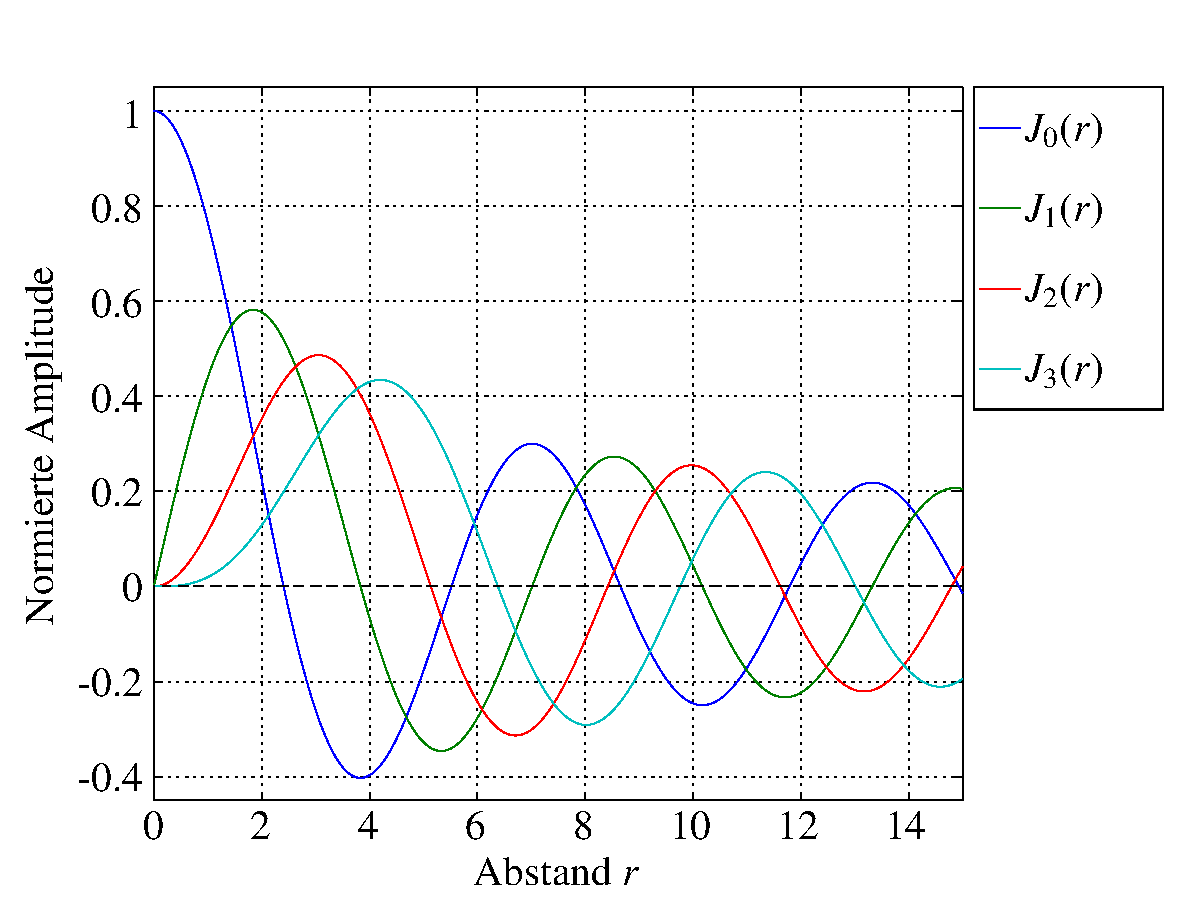
\includegraphics[scale=0.5]{kreis/besselfunction.pdf}
		\label{img:besselfunction}
		\caption[Besselfunktion]{Besselfunktion geplottet}
	\end{center}
\end{figure}

%\newpage
%
%\subsection{Veranschaulichung der Besselfunktion mit Beispielen}
%\begin{itemize}
%	\item Lautsprecher
%	\item Antenne
%	\item Lichtbrechung im Fernglas
%	\item \dots
%\end{itemize}